\documentclass{article}
\usepackage{amsmath}
\usepackage{amssymb}
\usepackage{graphicx}
\usepackage{hyperref}
\usepackage[version=4]{mhchem}

\title{Example 1}
\date{}

\begin{document}
\maketitle

Prove that the sum of any two sides of a triangle is greater than twice the length of median drawn to the third side.

Proof:
As shown in the figure, in \(\triangle A B C, A D\) is the median. We want to prove that \(A D<\frac{1}{2}(A B+A C)\).\\
\centering
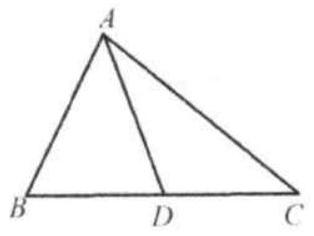
\includegraphics[width=\textwidth]{images/problem_image_1.jpg}

Extend \(A D\) to \(E\) such that \(A D=D E\).\\
Connect BE.

Since \(D E=A D, \angle B D E=\angle C D A . B D=D C\).\\
Thus \(\triangle B D E \cong \triangle C D A, B E=A C\),\\
In \(\triangle A B E, A B+B E>A E=2 A D\).\\
So \(A D<\frac{1}{2}(A B+B E)\).\\
\centering
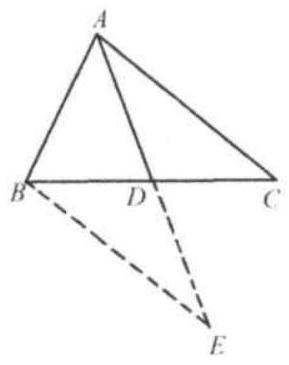
\includegraphics[width=\textwidth]{images/reasoning_image_1.jpg}

Since \(B E=A C\), we have \(A D<\frac{1}{2}(A B+A C)\).



\end{document}
